\chapter{问题分析和研究框架}
\label{cha:problem_framework}

\section{本章引论}

随着互联网上不同类型的平台出现,人们每天在各种平台上产生着各种各样的行为和发言。如现在微博平台上会对热门时事设置井号标签,人们透过加上对应标签来表达对该事件的想法,以及透过对这些发言进行赞点、分享或评论来表达支持或反驳。透过根据井号标签收集数据并进行意图分析可以得知网民对该事件的舆论方向。在其他平台上的各种行为记录同样可能有挖掘其意图的价值,意图识别的应用场景也变得多种多样,但即使数据的内容和结构不同,问题的本质是相似的。因此在本章,我们将首先针对意图识别进行分析,并给出统一的形式化表示。

再进一步,基于该形式化表示,我们提出一个面向社交媒体文本的意图识别研究框架。从原始文本的输入到最终识别目标的输出,理清其中每个步骤的功能和目的,给出一个完整识别系统的实现流程,为解决后续章节中研究的问题准备一个统一的切入点。

\section{问题分析}

本小节中,我们将对意图识别中涉及的各个元素作出分析,并给出统一的形式化表示来描述他们的相互关系。

不同意图识别问题中都有要被识别的意图倾向$C$。如Tang等人\cite{tang2015learning}的情感极性识别研究,$C$对应需要五级的情感极性。在刘丹丹等人\cite{刘丹丹2015基于}的微博情感分类研究中,$C$对应喜好、安乐、惊奇、厌恶、悲哀、愤恨、恐惧。邓钊等人\cite{2015面向微博的中文反语识别研究}的中文反语识别研究中,$C$则对应是否包含反讽。

其次是研究主体$T$,它是行为发起者$S$的行为记录,可以认为他表达想法和情感的载体。譬如要研究讨论区上帖子的意图倾向,那么$T$就是帖子的内容,包括其中的文本内容、图片、文件附件等,$S$则是帖子的发布者。另外一些场景下会有背景信息$B$,对应所有有助于正确理解$T$的信息,如帖子所在讨论区的类型有助于定位帖子对应的领域,发布者的发布历史显示发布者的一些态度倾向,帖子下的评论从侧表反映主帖的内容,这些都可能是理解帖子内容的提示。

意图识别假设对于任意一个研究样本$t \in T$,在给定背景信息$b \in B$(或某些情况下假设与背景信息无关),其承载想法或情感必然存在对应的倾向$c \in C$。意图识别首先要从样本主体和背景信息中分别提取出识别目标相关的信息$f_t$和$f_b$,即需要提出两个映射函数,$F_T$和$F_B$,满足 $f_t=F_T(t)$和$f_b=F_B(b)$。再进一步根据相关信息识别出其想法或情感倾向,即找出一个映射$F_C$,使得 $c=F_C(f_t, f_b)=F_C(F_T(t), F_B(b))$。

\section{框架设计}

在本小节,我们将根据前述的形式化表示给出一个意图识别的研究框架。由于在本论文的后续研究均面向英语难金社交媒体文本的分类问题,我们会针对此研究方法对框架进行细化,从原始文本的输入到最终识别目标的输出,理清其中每个步骤的功能和目的,给出一个完整系统的设计和实现流程。

\begin{figure}[H]
  \centering
  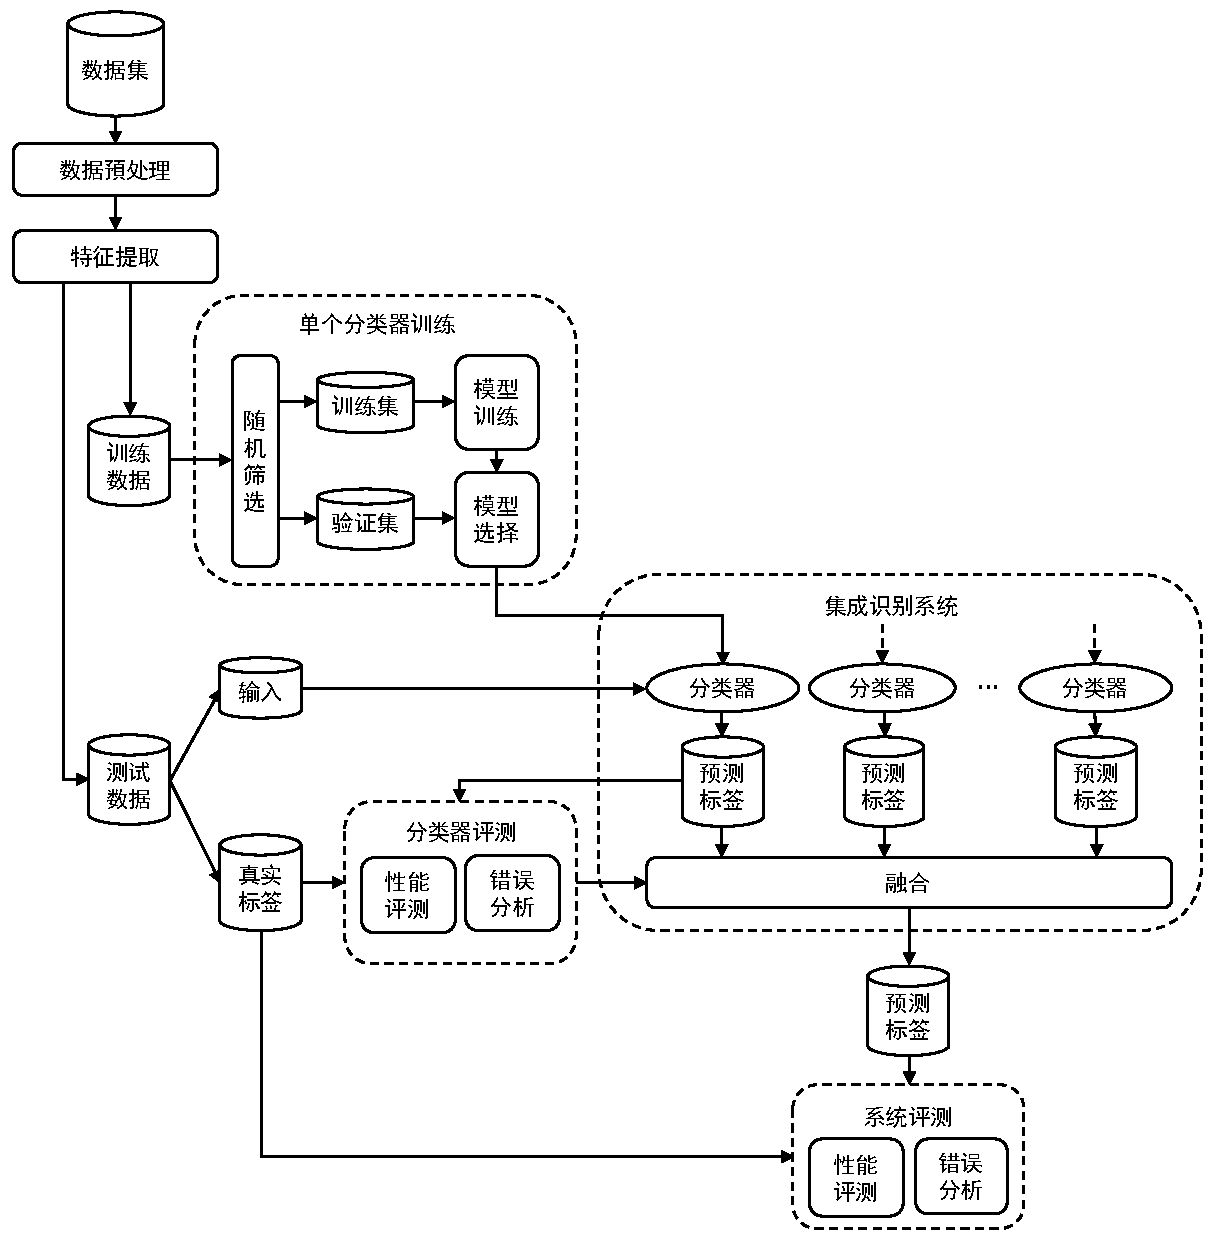
\includegraphics[width=\textwidth]{img/framework.pdf}
  \caption{意图识别的研究框架}
  \label{fig:framework}
\end{figure}

图~\ref{fig:framework}显示本文面向意图识别的研究框架。整个框架的输入是实验的数据集,数据集的每个样本包含三个元素,分别是研究的主体、背景信息和意图的倾向。参考前一小节的形式化表示,一个样本可以表示为 $<t, b, c> \in T \times B \times C$。不论是训练数据或测试数据,他们都采用相同的数据预处理技术和特征提取技术来获取样本的特征,以用作分类器的输入,即透过$F_T$和$F_B$分别获取$f_t=F_T(t)$和$f_b=F_B(b)$。

以研究集成识别系统为目标,我们先对基础分类器进行研究和分析,透过比较不同模型和不同参数在对应问题上的整体性能,决定最终组成集成系统的基础分类器的模型。对于机器学习方法,在模型的训练过程中,需要将训练数据会分成训练集和验证集两个部分。训练集用于调整模型的参数,根据预先设计的损失函数计算模型当前的预测结果和实际标签的偏差,透过微分计算出参数的调整方向,并以一定的学习步长逐步迭代。由于以上训练过程在数学逻辑上是以达到训练集上的最优解来调整参数,会出现在对训练样本过拟合的问题,因此会采用验证集来评估模型对训练集以外的样本的识别性能。在每一轮参数调整后计算当前模型在验证集上的性能指标,每一轮进行比较后从中选择最优的一轮参数作为该次模型训练最终的参数。

传统方法是取在验证集上目标指标达到最好的一组参数


\section{本章小结}

pass

